\sequence{Nombres réels et intervalles}{Réels et intervalles}{2--13 novembre 2026}
\section{Les ensembles de nombres}
\begin{cours}[Définitions]
\begin{itemize}
\item $\N$ : entiers naturels ; $\Z$ : entiers relatifs.
\item $\D$ : nombres décimaux, de la forme $a/10^n$ avec $a\in\Z$, $n\in\N$.
\item $\Q$ : nombres rationnels, de la forme $a/b$ avec $a,b\in\Z$, $b\ne0$.
\item $\R$ : nombres réels, représentés par les abscisses des points d'une droite graduée. Un réel non rationnel est \textbf{irrationnel}.
\end{itemize}
\[\N\subsetneq\Z\subsetneq\D\subsetneq\Q\subsetneq\R.\]
\end{cours}
\begin{center}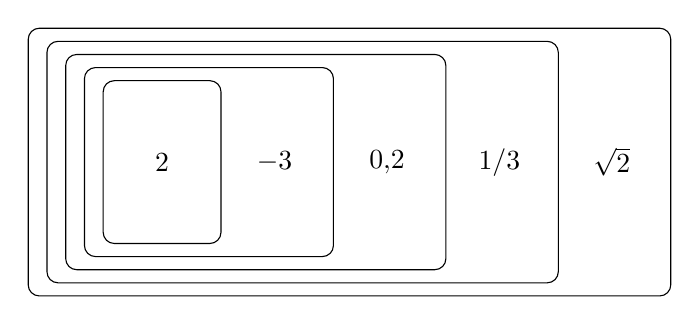
\begin{tikzpicture}[scale=.68]
\foreach \x/\w/\label in {0/12/\R,.35/9.9/\Q,.7/7.8/\D,1.05/5.7/\Z,1.4/3.6/\N}{\draw[rounded corners](\x,\x*.7)rectangle(\w,5-\x*.7);\node at(\w-.35,4.65-\x*.7){$\label$};}
\node at(2.5,2.5){$2$};\node at(4.6,2.5){$-3$};\node at(6.7,2.5){$0{,}2$};\node at(8.8,2.5){$1/3$};\node at(10.9,2.5){$\sqrt2$};
\end{tikzpicture}\end{center}
\ex{Donner le plus petit des cinq ensembles contenant chacun des nombres : $-95$ ; $7{,}29$ ; $5/3$ ; $\sqrt{25}$ ; $\sqrt2$ ; $\pi$ ; $0{,}0002$.}
\reponse[3.2]{$-95\in\Z$ ; $7{,}29\in\D$ ; $5/3\in\Q$ ; $\sqrt{25}=5\in\N$ ; $\sqrt2,\pi\in\R\setminus\Q$ ; $0{,}0002=2/10^4\in\D$. L'irrationalité de $\pi$ est admise ici.}

\fiche{Deux démonstrations par l'absurde}
\begin{methode}[Raisonnement par l'absurde]
Pour prouver une proposition, supposer sa négation, en déduire une contradiction, puis conclure que la proposition est vraie.
\end{methode}
\begin{cours}[Propriété]
$\dfrac13$ n'est pas un nombre décimal.
\end{cours}
\preuve[5]{Supposons $1/3=a/10^n$ avec $a\in\Z$, $n\in\N$. Alors $10^n=3a$ serait multiple de $3$. Pourtant $10\equiv1$ modulo $3$, donc $10^n$ a un reste de $1$ dans la division par $3$ (on peut aussi utiliser le critère de divisibilité par $3$). Contradiction. Donc $1/3\notin\D$.}
\begin{cours}[Propriété]
$\sqrt2$ est irrationnel.
\end{cours}
\preuve[6]{Supposons $\sqrt2=p/q$ avec $p,q\in\N$, $q\ne0$, et $p/q$ irréductible. Alors $p^2=2q^2$, donc $p^2$ est pair. Si $p$ était impair, son carré le serait aussi : ainsi $p$ est pair. Écrivons $p=2k$. On obtient $4k^2=2q^2$, puis $q^2=2k^2$ ; $q$ est donc pair à son tour. Ainsi $2$ divise $p$ et $q$, contrairement à l'irréductibilité. Donc $\sqrt2\notin\Q$.}
\prof{Faire identifier séparément l'hypothèse de départ, l'implication utilisée par contraposée sur la parité et la contradiction finale. Ne pas présenter une écriture décimale de calculatrice comme une preuve d'irrationalité.}

\fiche{Intervalles de la droite réelle}
\begin{cours}[Notations]
Pour deux réels $a<b$, les intervalles décrivent les réels compris entre deux bornes, avec ou sans les bornes. Un crochet fermé inclut la borne, un crochet ouvert l'exclut. Les symboles $-\infty,+\infty$ ne sont pas des réels et sont toujours accompagnés d'un crochet ouvert.
\end{cours}
\begin{center}\renewcommand{\arraystretch}{1.8}\begin{tabular}{c|c|l}
\textbf{Condition}&\textbf{Intervalle}&\textbf{Description}\\\hline
$a\leq x\leq b$&$[a;b]$&deux bornes incluses\\
$a<x\leq b$&$]a;b]$&$a$ exclu, $b$ inclus\\
$a\leq x<b$&$[a;b[$&$a$ inclus, $b$ exclu\\
$a<x<b$&$]a;b[$&deux bornes exclues\\
$x\geq a$&$[a;+\infty[$&supérieur ou égal à $a$\\
$x>a$&$]a;+\infty[$&strictement supérieur à $a$\\
$x\leq b$&$]-\infty;b]$&inférieur ou égal à $b$\\
$x<b$&$]-\infty;b[$&strictement inférieur à $b$
\end{tabular}\end{center}
\[\R=]-\infty;+\infty[,\quad \R^*=]-\infty;0[\,\cup\,]0;+\infty[.\]
\vigilance{Les réels strictement négatifs forment $]-\infty;0[$ : $0$ est exclu. $[a;a]=\{a\}$ ; $]a;a[=\varnothing$.}
\ex{Écrire sous forme d'intervalle puis représenter : $2\leq x\leq5$ ; $x>4$ ; $-6<x\leq2$ ; $x<0$.}
\reponse[4]{$[2;5]$ ; $]4;+\infty[$ ; $]-6;2]$ ; $]-\infty;0[$. Sur la droite graduée, indiquer les bornes, puis matérialiser chacune comme incluse ou exclue.}

\fiche{Intersection et réunion d'intervalles}
\begin{cours}[Définition]
$\,I\cap J$ correspond à la condition « appartenir à $I$ \textbf{et} à $J$ » ; $I\cup J$ correspond à « appartenir à $I$ \textbf{ou} à $J$ ». Une réunion d'intervalles n'est pas toujours un intervalle.
\end{cours}
\ex{Avec $I=[0;12]$ et $J=[3;20]$, déterminer $I\cap J$ et $I\cup J$.}
\reponse[2.4]{$I\cap J=[3;12]$ et $I\cup J=[0;20]$.}
\ex{Compléter, en justifiant par des représentations sur une droite graduée.}
\begin{center}\renewcommand{\arraystretch}{2}\begin{tabular}{c c|c c}
$I$&$J$&$I\cap J$&$I\cup J$\\\hline
$]-4;3]$&$[1;5]$&\trou{$[1;3]$}&\trou{$]-4;5]$}\\
$]-\infty;2]$&$[-4;+\infty[$&\trou{$[-4;2]$}&\trou{$\R$}\\
$]-\infty;7]$&$[7;+\infty[$&\trou{$\{7\}$}&\trou{$\R$}\\
$]-\infty;5]$&$[-3;+\infty[$&\trou{$[-3;5]$}&\trou{$\R$}\\
$]-2;0[$&$]0;3]$&\trou{$\varnothing$}&\trou{$]-2;0[\cup]0;3]$}
\end{tabular}\end{center}
\reponse[4]{Pour chaque intersection, conserver les points communs aux deux représentations ; pour chaque réunion, conserver tous les points de l'une au moins. Dans la dernière ligne, $0$ n'appartient à aucun intervalle : on ne peut pas remplacer la réunion par $]-2;3]$.}
\rituel{Simplifier $\vect{AB}+\vect{BC}$ ; résoudre $3x-6=0$ ; calculer $10^{-2}$.}{$\vect{AC}$ ; $x=2$ ; $0{,}01$.}

\fiche{Valeur absolue et distance}
\begin{cours}[Définition et propriétés]
$|x|$ est la distance du réel $x$ à $0$ ; $|x|\geq0$ et
\[|x|=\begin{cases}x&\text{si }x\geq0,\\-x&\text{si }x<0.\end{cases}\]
La distance entre $a$ et $b$ est $|b-a|$. Pour $a\in\R$ et $r\geq0$ :
\[|x-a|\leq r\iff x\in[a-r;a+r],\qquad |x-a|<r\iff x\in]a-r;a+r[.\]
\end{cours}
\ex{Calculer $|3{,}2|$, $|-1{,}6|$, $|\sqrt3-2|$, puis les distances entre $2$ et $5$, $2$ et $-5$, $-2$ et $-5$.}
\reponse[2.4]{$3{,}2$ ; $1{,}6$ ; $2-\sqrt3$ puisque $\sqrt3<2$. Les distances sont $3$, $7$ et $3$.}
\ex{Résoudre : $|x-7/3|=14$ ; $|x-2|\leq3$ ; $|x+3|<5$.}
\reponse[4.8]{Pour la première équation, $x-7/3=14$ ou $x-7/3=-14$, donc $S=\{-35/3;49/3\}$. Puis $|x-2|\leq3\iff x\in[-1;5]$. Enfin $|x+3|=|x-(-3)|<5\iff x\in]-8;2[$.}
\ex{Écrire $x\in[4;10]$ sous forme d'une inégalité avec valeur absolue.}
\reponse[2]{Le centre est $(4+10)/2=7$ et le rayon $(10-4)/2=3$ : $|x-7|\leq3$.}

\fiche{Encadrements et approximations}
\begin{cours}[Vocabulaire]
Encadrer $x$, c'est donner $a\leq x\leq b$ ; l'amplitude est $b-a$. Une valeur approchée par défaut est inférieure ou égale à $x$ ; une valeur approchée par excès lui est supérieure ou égale. L'arrondi choisit la valeur la plus proche à la précision demandée.
Les chiffres significatifs se comptent à partir du premier chiffre non nul ; la précision affichée doit convenir au contexte.
\end{cours}
\ex{Encadrer $\sqrt2$ par deux centièmes consécutifs. Donner son arrondi au centième. Arrondir $0{,}004567$ à trois chiffres significatifs, puis $12345$ à trois chiffres significatifs en écriture scientifique.}
\reponse[3.2]{$1{,}41^2=1{,}9881<2<2{,}0164=1{,}42^2$, donc $1{,}41<\sqrt2<1{,}42$ (amplitude $0{,}01$). L'arrondi au centième est $1{,}41$. Les autres arrondis sont $0{,}00457$ et $1{,}23\times10^4$.}
\begin{lstlisting}
def encadre_racine2(p):
    # p entier naturel ; calculs entiers exacts
    q = 10**p
    k = 0
    while (k+1)**2 <= 2*q*q:
        k = k+1
    return k/q, (k+1)/q
\end{lstlisting}
\ex{Expliquer pourquoi cette fonction encadre $\sqrt2$. Que renvoie-t-elle pour $p=2$ ? Pourquoi termine-t-elle ?}
\reponse[3.2]{La boucle cherche le plus grand entier $k$ tel que $k^2\leq2q^2$. À la sortie, $k^2\leq2q^2<(k+1)^2$, donc $k/q\leq\sqrt2<(k+1)/q$. Pour $p=2$, elle renvoie $(1{,}41;1{,}42)$. Comme $(2q)^2>2q^2$, le compteur finit par atteindre une valeur qui rend le test faux. Les divisions finales sont des approximations flottantes ; les tests de carrés sont exacts.}
